%
% Main document
% ===========================================================================
% This is part of the document "Project documentation template".
% Authors: brd3, kaa1
%

%---------------------------------------------------------------------------
\documentclass[
	a4paper,					% paper format
	12pt,							% fontsize
	oneside,					% double-sided
	openany,				% begin new chapter on right side
	notitlepage,			% use no standard title page
	parskip=half,			% set paragraph skip to half of a line
]{scrreprt}					% KOMA-script report
%---------------------------------------------------------------------------

\raggedbottom
\KOMAoptions{cleardoublepage=plain}			% Add header and footer on blank pages


% Load Standard Packages:
%---------------------------------------------------------------------------
\usepackage[standard-baselineskips]{cmbright}
\usepackage[ngerman,english]{babel}										% english hyphenation
%\usepackage[latin1]{inputenc}  							% Unix/Linux - load extended character set (ISO 8859-1)
\usepackage[ansinew]{inputenc}  							% Windows - load extended character set (ISO 8859-1)
\usepackage[T1]{fontenc}											% hyphenation of words with �,� and �
\usepackage{textcomp}													% additional symbols
\usepackage{ae}																% better resolution of Type1-Fonts 
\usepackage{fancyhdr}													% simple manipulation of header and footer 
\usepackage{etoolbox}													% color manipulation of header and footer
\usepackage{graphicx}                      		% integration of images
\usepackage{float}														% floating objects
\usepackage{caption}													% for captions of figures and tables
\DeclareCaptionLabelFormat{blank}{}
\usepackage{booktabs}													% package for nicer tables
\usepackage{tocvsec2}													% provides means of controlling the sectional numbering
\usepackage{pgfgantt}
\usepackage{graphicx}
\usepackage{xcolor}
\usepackage{pdflscape}
\usepackage{setspace}
\usepackage{rotating}

%---------------------------------------------------------------------------

% Load Math Packages
%---------------------------------------------------------------------------
\usepackage{amsmath}                    	   	% various features to facilitate writing math formulas
\usepackage{amsthm}                       	 	% enhanced version of latex's newtheorem
\usepackage{amsfonts}                      		% set of miscellaneous TeX fonts that augment the standard CM
\usepackage{amssymb}													% mathematical special characters
\usepackage{exscale}													% mathematical size corresponds to textsize
%---------------------------------------------------------------------------

% Package to facilitate placement of boxes at absolute positions
%---------------------------------------------------------------------------
\usepackage[absolute]{textpos}
\setlength{\TPHorizModule}{1mm}
\setlength{\TPVertModule}{1mm}
%---------------------------------------------------------------------------					
			
% Definition of Colors
%---------------------------------------------------------------------------
\RequirePackage{color}                          % Color (not xcolor!)
\definecolor{linkblue}{rgb}{0,0,0.8}            % Standard
\definecolor{darkblue}{rgb}{0,0.08,0.45}        % Dark blue
\definecolor{bfhgrey}{rgb}{0.41,0.49,0.57}      % BFH grey
%\definecolor{linkcolor}{rgb}{0,0,0.8}     			% Blue for the web- and cd-version!
\definecolor{linkcolor}{rgb}{0,0,0}        			% Black for the print-version!
%---------------------------------------------------------------------------

% Hyperref Package (Create links in a pdf)
%---------------------------------------------------------------------------
\usepackage[
	pdftex,ngerman,bookmarks,plainpages=false,pdfpagelabels,
	backref = {false},										% No index backreference
	colorlinks = {true},                  % Color links in a PDF
	hypertexnames = {true},               % no failures "same page(i)"
	bookmarksopen = {true},               % opens the bar on the left side
	bookmarksopenlevel = {0},             % depth of opened bookmarks
	pdftitle = {Preliminary_Study_Rob195},	   	% PDF-property
	pdfauthor = {aescd1},        					  % PDF-property
	pdfsubject = {LaTeX Template},        % PDF-property
	linkcolor = {linkcolor},              % Color of Links
	citecolor = {linkcolor},              % Color of Cite-Links
	urlcolor = {linkcolor},               % Color of URLs
]{hyperref}
%---------------------------------------------------------------------------

% Set up page dimension
%---------------------------------------------------------------------------
\usepackage{geometry}
\geometry{
	a4paper,
	left=28mm,
	right=15mm,
	top=30mm,
	headheight=10mm,
	headsep=10mm,
	textheight=242mm,
	footskip=15mm
}
%---------------------------------------------------------------------------

% Makeindex Package
%---------------------------------------------------------------------------
\usepackage{makeidx}                         		% To produce index
\makeindex                                    	% Index-Initialisation
%---------------------------------------------------------------------------

% Glossary Package
%---------------------------------------------------------------------------
% the glossaries package uses makeindex
% if you use TeXnicCenter do the following steps:
%  - Goto "Ausgabeprofile definieren" (ctrl + F7)
%  - Select the profile "LaTeX => PDF"
%  - Add in register "Nachbearbeitung" a new "Postprozessoren" point named Glossar
%  - Select makeindex.exe in the field "Anwendung" ( ..\MiKTeX x.x\miktex\bin\makeindex.exe )
%  - Add this [ -s "%tm.ist" -t "%tm.glg" -o "%tm.gls" "%tm.glo" ] in the field "Argumente"
%
% for futher informations go to http://ewus.de/tipp-1029.html
%---------------------------------------------------------------------------
\usepackage[nonumberlist]{glossaries}
\makeglossaries

\newglossaryentry{BibTeX}{name={BibTeX},description={Program for the creation of 	bibliographical references and directories in \TeX or \LaTeX documents}}
\newglossaryentry{Index}{name={Index},description={Index with keywords from text}}



%---------------------------------------------------------------------------

% Intro:
%---------------------------------------------------------------------------
\begin{document} 									                     	% Start Document
\setstretch{1.25}
\color{black}
\settocdepth{section}														% Set depth of toc
\pagenumbering{roman}														
%---------------------------------------------------------------------------

\providecommand{\heading}{Title of Thesis}		%  Insert Title of Thesis here					% Titel der Arbeit aus Datei titel.tex lesen
\providecommand{\versionnumber}{1.2}			%  Hier die aktuelle Versionsnummer eingeben
\providecommand{\versiondate}{07.02.2014}		%  Hier das Datum der aktuellen Version eingeben				% Versionsnummer und -datum aus Datei version.tex lesen

% Set up header and footer
%---------------------------------------------------------------------------
\makeatletter
\patchcmd{\@fancyhead}{\rlap}{\color{bfhgrey}\rlap}{}{}		% new color of header
\patchcmd{\@fancyfoot}{\rlap}{\color{bfhgrey}\rlap}{}{}		% new color of footer
\makeatother

\fancyhf{}																		% clean all fields
\fancypagestyle{plain}{												% new definition of plain style	
	\fancyfoot[OR,EL]{\footnotesize \thepage} 	% footer right part --> page number
	\fancyfoot[OL,ER]{\footnotesize \heading, Version \versionnumber, \versiondate}	% footer even page left part 
}

\renewcommand{\chaptermark}[1]{\markboth{\thechapter.  #1}{}}
\renewcommand{\headrulewidth}{0pt}				% no header stripline
\renewcommand{\footrulewidth}{0pt} 				% no bottom stripline

\pagestyle{plain}
%---------------------------------------------------------------------------


% Title Page and Abstract
%---------------------------------------------------------------------------
%%
% Project documentation template
% ===========================================================================
% This is part of the document "Project documentation template".
% Authors: brd3, kaa1
%

\begin{titlepage}


% BFH-Logo absolute placed at (28,12) on A4 and picture (16:9 or 15cm x 8.5cm)
% Actually not a realy satisfactory solution but working.
%---------------------------------------------------------------------------
\setlength{\unitlength}{1mm}
\begin{textblock}{20}[0,0](28,12)
	
\includegraphics[scale=1.0]{images/BFH_Logo_B.png}
\end{textblock}

% Institution / titel / subtitel / authors / experts:
%---------------------------------------------------------------------------
\begin{flushleft}

\vspace*{21mm}

\fontsize{26pt}{40pt}\selectfont 
\heading				\\							% Read heading from file leader/title.tex
\vspace{2mm}

\fontsize{16pt}{24pt}\selectfont\vspace{0.3em}
Place your subheading here 			\\				% Insert subheading
\vspace{5mm}

\fontsize{10pt}{12pt}\selectfont
\textbf{Description of thesis (semester- / Bachelor thesis / etc.)} \\		% Insert text
\vspace{7mm}

% Abstract (eingeben):
%---------------------------------------------------------------------------
\begin{textblock}{150}(28,100)
\fontsize{10pt}{12pt}\selectfont
[Insert short text (abstract) if desired] \\ 
This document serves as a template for the compilation of reports according to the guidelines of the BFH. The template is written in LATEX and supports the automatic writing of various directories, references, indexing and glossaries. This small text is a summary of this document with a length of 4 to max. 8 lines. \\ 
The cover picture may be turned on or off in the lines 157/158 of the file template.tex.
\end{textblock}

\begin{textblock}{150}(28,225)
\fontsize{10pt}{17pt}\selectfont
\begin{tabbing}
xxxxxxxxxxxxxxx\=xxxxxxxxxxxxxxxxxxxxxxxxxxxxxxxxxxxxxxxxxxxxxxx \kill
Degree course:	\> [z.B. Electrical and Communication Engineering]	\\		% insert name of degree course
Authors:		\> [Test Peter, M\"uster R\"os\"a]		\\					% insert names
Tutor:	\> [Dr.~Xxxx Xxxx, Dr.~Yyyy Yyyy]		\\							% insert names
Constituent:	\> [Wwwww AG]					\\							% insert names
Experts:		\> [Dr.~Zzzz Zzzz]				\\							% insert names
Date:			\> \versiondate					\\							% read from file leader/version.tex
\end{tabbing}

\end{textblock}
\end{flushleft}

\begin{textblock}{150}(28,280)
\noindent 
\color{bfhgrey}\fontsize{9pt}{10pt}\selectfont
Berner Fachhochschule | Haute \'ecole sp\'ecialis\'ee bernoise | Bern University of Applied Sciences
\color{black}\selectfont
\end{textblock}


\end{titlepage}

%
% ===========================================================================
% EOF
%
		% activate for frontpage without picture
%
% Project documentation template
% ===========================================================================
% This is part of the document "Project documentation template".
% Authors: brd3, kaa1
%

\begin{titlepage}


% BFH-Logo absolute placed at (28,12) on A4 and picture (16:9 or 15cm x 8.5cm)
% Actually not a realy satisfactory solution but working.
%---------------------------------------------------------------------------
\setlength{\unitlength}{1mm}
\begin{textblock}{20}[0,0](28,12)
	
\includegraphics[scale=1.0]{images/BFH_Logo_B.png}
\end{textblock}

\begin{textblock}{154}(28,48)
	\begin{picture}(150,2)
		\put(0,0){\color{bfhgrey}\rule{150mm}{2mm}}
	\end{picture}
\end{textblock}

\begin{textblock}{154}[0,0](28,51)
	\begin{figure}
	\centering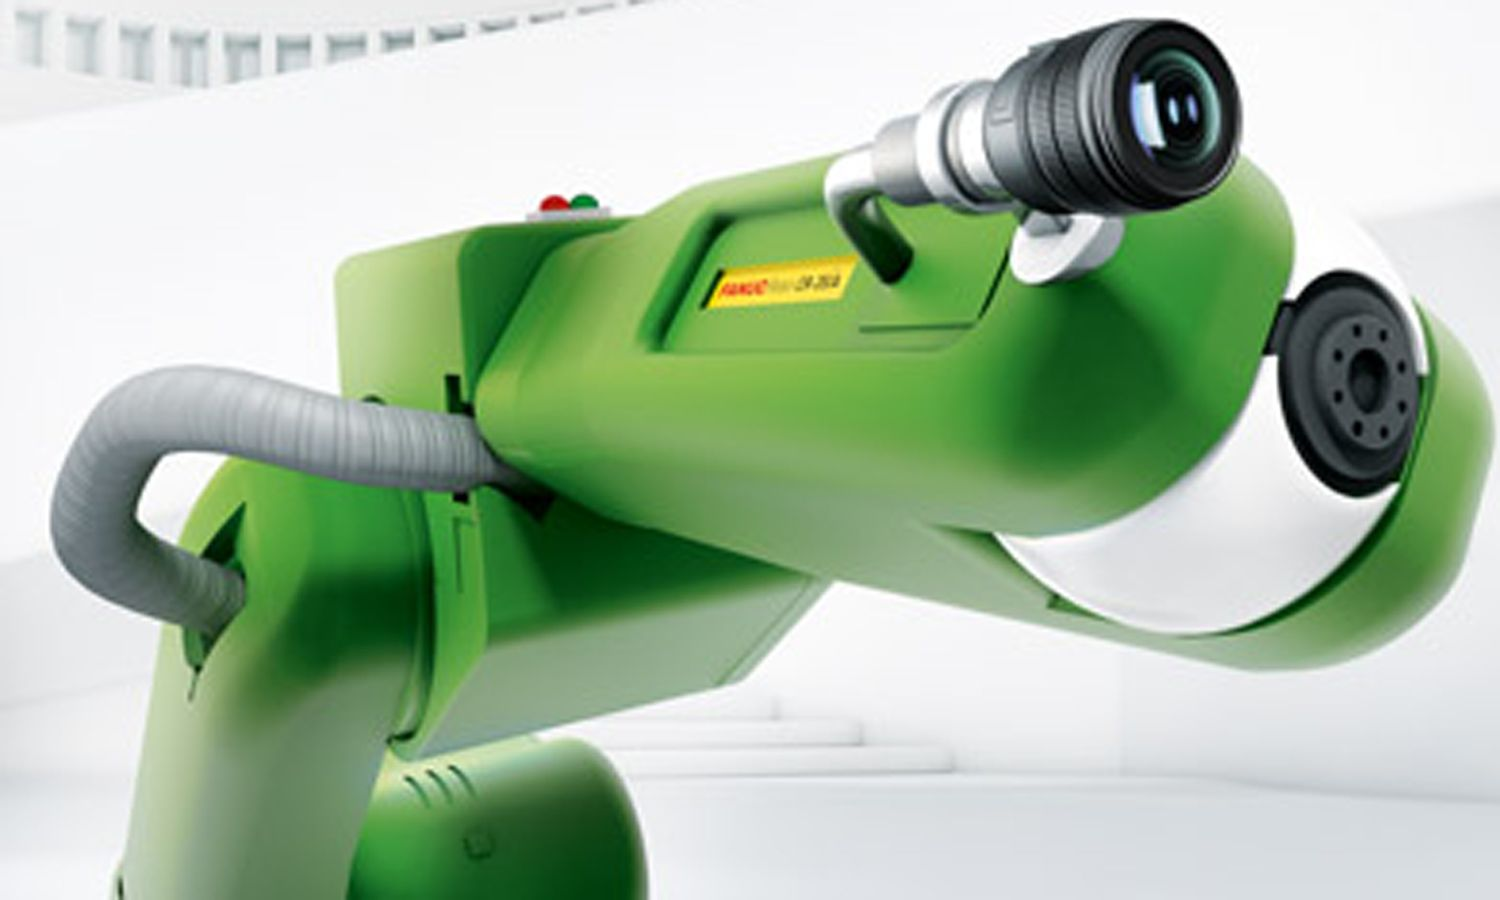
\includegraphics[scale=0.26]{images/fanuc_close.jpg}			% define cover picture
	\captionsetup{textformat=empty,labelformat=blank}
	\caption{Frontpage Picture \cite{fig:frontpage}}
	\end{figure}
\end{textblock}

\begin{textblock}{154}(28,133)
	\begin{picture}(150,2)
		\put(0,0){\color{bfhgrey}\rule{150mm}{2mm}}
	\end{picture}
\end{textblock}
\color{black}

% Institution / titel / subtitel / authors / experts:
%---------------------------------------------------------------------------
\begin{flushleft}

\vspace*{115mm}

\fontsize{26pt}{28pt}\selectfont 
\heading				\\							% Read heading from file leader/title.tex
\vspace{2mm}

\fontsize{16pt}{20pt}\selectfont\vspace{0.3em}
Preliminary Studies of Bachelor Thesis Rob195		\\				% Insert subheading
\vspace{5mm}

%\fontsize{10pt}{12pt}\selectfont
%\textbf{Description of thesis (semester- / Bachelor thesis / etc.)} \\		% Insert text
%\vspace{3mm}

% Abstract (eingeben):
%---------------------------------------------------------------------------
%\begin{textblock}{150}(28,190)
%\fontsize{10pt}{12pt}\selectfont
%[Insert short text (abstract) if desired] \\ 
%This document serves as a template for the compilation of reports according to the guidelines of the BFH. The template is written in LATEX and supports the automatic writing of various directories, references, indexing and glossaries. This small text is a summary of this document with a length of 4 to max. 8 lines. \\ 
%The cover picture may be turned on or off in the lines 157/158 of the file template.tex.
%\end{textblock}

\begin{textblock}{150}(28,225)
\fontsize{10pt}{17pt}\selectfont
\begin{tabbing}
	xxxxxxxxxxxxxxx\=xxxxxxxxxxxxxxxxxxxxxxxxxxxxxxxxxxxxxxxxxxxxxxx \kill
	Degree course:	\> Micro and Medical Technologies	\\		% insert name of degree course
	Author:		\> Aeschlimann Dario		\\					% insert names
	Tutors:	\> Rochat Sarah, Gruener Gabriel		\\							% insert names
	Constituent:	\> AHB Biel					\\							% insert names
	Experts:		\> Aigner Nikita				\\							% insert names
	Date:			\> \versiondate					\\							% read from file leader/version.tex
\end{tabbing}

\end{textblock}
\end{flushleft}

\begin{textblock}{150}(28,280)
\noindent 
\color{bfhgrey}\fontsize{9pt}{10pt}\selectfont
Berner Fachhochschule | Haute \'ecole sp\'ecialis\'ee bernoise | Bern University of Applied Sciences
\color{black}\selectfont
\end{textblock}


\end{titlepage}

%
% ===========================================================================
% EOF
%
		% activate for frontpage with picture
\cleardoubleemptypage
\setcounter{page}{1}
%\cleardoublepage
\phantomsection 

\chapter*{Management Summary}
\label{chap:managementSummary}

Lorem ipsum dolor sit amet, consectetur adipiscing elit. Phasellus scelerisque, leo sed iaculis ornare, mi leo semper urna, ac elementum libero est at risus. Donec eget aliquam urna. Lorem ipsum dolor sit amet, consectetur adipiscing elit. Nunc fermentum nunc sollicitudin leo porttitor volutpat. Duis ac enim lectus, quis malesuada lectus. Aenean vestibulum suscipit justo, in suscipit augue venenatis a. Donec interdum nibh ligula. Aliquam vitae dui a odio cursus interdum quis vitae mi. Phasellus ornare tortor fringilla velit accumsan quis tincidunt magna eleifend. Praesent nisl nibh, cursus in mattis ac, ultrices ac nulla. Nulla ante urna, aliquet eu tempus ut, feugiat id nisl. Nunc sit amet mauris vitae turpis scelerisque mattis et sed metus. Aliquam interdum congue odio, sed semper elit ullamcorper vitae. Morbi orci elit, feugiat vel hendrerit nec, sollicitudin non massa. Quisque lacus metus, vulputate id ullamcorper id, consequat eget orci \nocite{kopka:band1} \nocite{Marti06}. 

\cleardoubleemptypage
%---------------------------------------------------------------------------

% Table of contents
%---------------------------------------------------------------------------
\tableofcontents
%\cleardoublepage
%---------------------------------------------------------------------------

% Main part:
%---------------------------------------------------------------------------
\pagenumbering{arabic}
\setstretch{1.25}
\chapter{Introduction}
\label{chap:introduction}
\setstretch{1.5}
Collaborative robots are meant to be flexible and easy to be reprogrammed so that they can be used efficiently in the modern industrial environment. One of the most important aspects for collaborative robots is safety. The robot shall not cause any harm to people or material. 
Currently there are three different types \cite{robotiq}  how the workspace of robots is monitored and protected from collisions:

\begin{itemize}
	\item Safety monitored stop: Scanners detect humans and objects inside the workspace of the robot and force a stop of any robot motion. This means the robot is not collaborative.
	\item Speed and separation monitoring: Scanners detect humans and objects inside certain areas around the robot and adjust the speed of the robot when the human comes closer to the robot. This leads to a stop of any robot motion when the human is coming too close to the robot. This is also referred to as cooperative operation.
	\item Power and force limiting: The robot is equipped with force and torque sensor to detect any abnormal forces applied to the robot body. Detecting such a force leads to a stop any robot motion. This type is called collaborative robot.Collisions can also be detected via a  sensitive skin on the robot. The skins can be pressure sensisitive or capacitive. The latter can detect flesh (they typically can not differentiate between a living human and a sausage) within a cm or two next to the skin. 
\end{itemize}
	
%	https://blog.robotiq.com/what-does-collaborative-robot-mean
Robots that rely on force sensors to detect collisions only recognize them and thus stopping any motion when the collision is already taking place. In a collaborative situation, the robot acts within a dynamic workspace and containers with liquids or heavy unstable objects may obstruct the workspace. These objects may be tipped over by the robot without triggering a halt or the halt could be triggered too late based on the force sensors, which could pose a health risk.
In addition, halts caused by the force sensors cause downtime in the production process which leads to higher production costs and longer production times, which companies like to avoid.
The goal of this thesis is to develop a vision system, which detects in real-time any occupied area in the workspace, that means people or objects which are within reach of the robot, and adapts the robots trajectories to avoid any collisions, thus providing an extra layer of safety. This would allow the robot to work in a modifiable workspace together with a human and to adapt his movements according to the human ones \cite{work_desc}. 

GPU-Voxels \cite{GPU-Voxels} is a similar project, that already has a vision system implemented to monitor the surroundings of various robots. It is mostly used in mobile robotics but has some implementations with an collaborative robots.

Commercially available camera based systems like the Pilz SafetyEye \cite{pilz} can recognize changes in the robot environment, however they do not have any capabilities to modify the robot's path.


\chapter{Tools}
\label{chap:tools}
\setstretch{1.5}
\section{Hardware & Software}
\label{sec: hwsw}
Fanuc CR35-iA Robot

Asus Xtion Pro Live

Roboguide

\section{Libraries and Algorithms}
\label{sec:libalg}

Point Cloud Library:
-Description
-Usage
-possibilities

Octomap:
-Description
-Usage
-possibilities





\chapter{Planning of the preliminary study}
\label{chap:Planning}
\setstretch{1.5}
The first step of this preliminary study was to plan, how to attempt this project. A plan and a timetable had to be created by taking in account the given work specification \cite{work_desc}. These work specifications defined the following goals for the preliminary study.
\setstretch{1.0}
\begin{itemize}
	\item Write specification, test and validation plan.
	\item Perform a literature review.
	\item Select, order and commission parts for test setup.
	\item get familiarized with robot system and Interface.
	\item Integrate a model of the robot in the collision-avoidance software.
	\item Generate a project plan for the thesis.
\end{itemize}
\setstretch{1.5}

The procedure was planned according these goals by giving them a timely order and a duration per task. This plan was implemented in a Gantt chart which is shown in figure \ref{fig:gantt}.
During the execution of this preliminary study, the plan has been adapted to the current state of the work.

As planned, the literature review started right away but takes place over the whole preliminary study, as there will always be some topics that need further research. The research has been done online by using forums and library and program documentations.
Next to the research, the system specification has been one of the first tasks to approach, due to the reason that the specifications build the fundament for the implementation. When system specifications are defined, an according test to validate the system shall be defined and documented. These tests allow to define measurable goals for each implemented specification as the test can be either successful or not. With this information the validation can be carried out. While finishing the test and validation plan, the author must get acquainted with the robot system and its interface.


While getting familiar with the robot system, a decision about the needed hardware components need to be taken. It's important to choose the parts in an early stage of time as they may need some time to be delivered. All components need to be available in week 12 of the project, so that they can be used when the Bachelor Thesis starts.


A big amount of time is planned for the implementation of the robot model. The goal of this implementation is, that the planning of the thesis can be done basing on the progress of this implementation. So the further this implementation is along, the more detailed and realistic the planning of the Thesis can be foreseen.

The Last Week of the preliminary study acts as buffer zone, with reserved time for proofreading and finishing the documentation.
%\section{Timetable}
\begin{landscape}
\begin{figure}[h]
\centering
\begin{ganttchart}[%Specs
y unit title=0.6cm,
y unit chart=0.8cm,
x unit = 0.28cm,
vgrid={*4{black,dotted},*3{red,dashed}},hgrid={black,thin},
title height=1,
newline shortcut=true,
bar label node/.append style={align=left},
%     title/.style={fill=none},
title label font=\bfseries\footnotesize,
bar/.style={fill=blue},
bar height=0.6,
bar top shift=0.2,
%   progress label text={},
group right shift=0,
group top shift=0.8,
group height=.2,
group peaks width={0.4},
inline=false]{1}{77}
%labels
\gantttitle{\textbf{Bachelor Thesis Rob195, Preliminary Studies}}{77}\\  	% title 1
%    \gantttitle[]{Preliminary Studies}{11}     	% title 2
%    \gantttitle[]{Thesis}{11} \\         		% title 3     
\gantttitle{PW1}{7}
\gantttitle{PW2}{7}
\gantttitle{PW3}{7}  
\gantttitle{PW4}{7}  
\gantttitle{PW5}{7}  
\gantttitle{PW6}{7}  
\gantttitle{PW7}{7}  
\gantttitle{PW8}{7}  
\gantttitle{PW9}{7}  
\gantttitle{PW10}{7}  
\gantttitle{PW11}{7}\\
%    dates
\gantttitle{18.2.-24.2.}{7}
\gantttitle{25.2.-03.3.}{7}
\gantttitle{4.3.-10.3.}{7}  
\gantttitle{11.3.-17.3.}{7}  
\gantttitle{18.3.-24.3}{7}  
\gantttitle{25.3.-31.3.}{7}  
\gantttitle{1.4.-7.4.}{7}  
\gantttitle{8.4.-14.4.}{7}  
\gantttitle{15.4.-21.4.}{7}  
\gantttitle{22.4.-28.4.}{7}  
\gantttitle{29.4.-5.5.}{7}\\
%    Week 1
\gantttitle{\rotatebox{90}{M}}{1}
\gantttitle{\rotatebox{90}{T}}{1}  
\gantttitle{\rotatebox{90}{W}}{1}  
\gantttitle{\rotatebox{90}{Th}}{1}  
\gantttitle{\rotatebox{90}{F}}{1}  
\gantttitle{\rotatebox{90}{S}}{1}  
\gantttitle{\rotatebox{90}{Su}}{1}
%    Week 2
 \gantttitle{\rotatebox{90}{M}}{1}
\gantttitle{\rotatebox{90}{T}}{1}  
\gantttitle{\rotatebox{90}{W}}{1}  
\gantttitle{\rotatebox{90}{Th}}{1}  
\gantttitle{\rotatebox{90}{F}}{1}  
\gantttitle{\rotatebox{90}{S}}{1}  
\gantttitle{\rotatebox{90}{Su}}{1} 
%    Week 3
 \gantttitle{\rotatebox{90}{M}}{1}
\gantttitle{\rotatebox{90}{T}}{1}  
\gantttitle{\rotatebox{90}{W}}{1}  
\gantttitle{\rotatebox{90}{Th}}{1}  
\gantttitle{\rotatebox{90}{F}}{1}  
\gantttitle{\rotatebox{90}{S}}{1}  
\gantttitle{\rotatebox{90}{Su}}{1}
%    Week 4
 \gantttitle{\rotatebox{90}{M}}{1}
\gantttitle{\rotatebox{90}{T}}{1}  
\gantttitle{\rotatebox{90}{W}}{1}  
\gantttitle{\rotatebox{90}{Th}}{1}  
\gantttitle{\rotatebox{90}{F}}{1}  
\gantttitle{\rotatebox{90}{S}}{1}  
\gantttitle{\rotatebox{90}{Su}}{1} 
%    Week 5
 \gantttitle{\rotatebox{90}{M}}{1}
\gantttitle{\rotatebox{90}{T}}{1}  
\gantttitle{\rotatebox{90}{W}}{1}  
\gantttitle{\rotatebox{90}{Th}}{1}  
\gantttitle{\rotatebox{90}{F}}{1}  
\gantttitle{\rotatebox{90}{S}}{1}  
\gantttitle{\rotatebox{90}{Su}}{1} 
%    Week 6
 \gantttitle{\rotatebox{90}{M}}{1}
\gantttitle{\rotatebox{90}{T}}{1}  
\gantttitle{\rotatebox{90}{W}}{1}  
\gantttitle{\rotatebox{90}{Th}}{1}  
\gantttitle{\rotatebox{90}{F}}{1}  
\gantttitle{\rotatebox{90}{S}}{1}  
\gantttitle{\rotatebox{90}{Su}}{1} 
%    Week 7
 \gantttitle{\rotatebox{90}{M}}{1}
\gantttitle{\rotatebox{90}{T}}{1}  
\gantttitle{\rotatebox{90}{W}}{1}  
\gantttitle{\rotatebox{90}{Th}}{1}  
\gantttitle{\rotatebox{90}{F}}{1}  
\gantttitle{\rotatebox{90}{S}}{1}  
\gantttitle{\rotatebox{90}{Su}}{1} 
%    Week 8
 \gantttitle{\rotatebox{90}{M}}{1}
\gantttitle{\rotatebox{90}{T}}{1}  
\gantttitle{\rotatebox{90}{W}}{1}  
\gantttitle{\rotatebox{90}{Th}}{1}  
\gantttitle{\rotatebox{90}{F}}{1}  
\gantttitle{\rotatebox{90}{S}}{1}  
\gantttitle{\rotatebox{90}{Su}}{1} 
%    Week 9
 \gantttitle{\rotatebox{90}{M}}{1}
\gantttitle{\rotatebox{90}{T}}{1}  
\gantttitle{\rotatebox{90}{W}}{1}  
\gantttitle{\rotatebox{90}{Th}}{1}  
\gantttitle{\rotatebox{90}{F}}{1}  
\gantttitle{\rotatebox{90}{S}}{1}  
\gantttitle{\rotatebox{90}{Su}}{1} 
%    Week 10
 \gantttitle{\rotatebox{90}{M}}{1}
\gantttitle{\rotatebox{90}{T}}{1}  
\gantttitle{\rotatebox{90}{W}}{1}  
\gantttitle{\rotatebox{90}{Th}}{1}  
\gantttitle{\rotatebox{90}{F}}{1}  
\gantttitle{\rotatebox{90}{S}}{1}  
\gantttitle{\rotatebox{90}{Su}}{1} 
%    Week 11
 \gantttitle{\rotatebox{90}{M}}{1}
\gantttitle{\rotatebox{90}{T}}{1}  
\gantttitle{\rotatebox{90}{W}}{1}  
\gantttitle{\rotatebox{90}{Th}}{1}  
\gantttitle{\rotatebox{90}{F}}{1}  
\gantttitle{\rotatebox{90}{S}}{1}  
\gantttitle{\rotatebox{90}{Su}}{1}                         
%    \gantttitle{TW1}{1}
%    \gantttitle{TW2}{1} 
%    \gantttitle{TW3}{1} 
%    \gantttitle{TW4}{1} 
%    \gantttitle{TW5}{1} 
%    \gantttitle{TW6}{1} 
%    \gantttitle{TW7}{1} 
%    \gantttitle{TW8}{1}   

% Setting group if any
\ganttgroup[inline=false]{Planning}{1}{35}\\ 
\ganttbar[progress=100,inline=false]{System Specification}{1}{23}\\
\ganttbar[progress=100,inline=false]{Test and Validation\ganttalignnewline Plan}{15}{33}\\
\ganttbar[progress=80,inline=false]{Literature Review}{1}{70}\\
\ganttbar[progress=80,inline=false]{Robot System and\ganttalignnewline Interface, Learning}{22}{33}\\
\ganttbar[progress=100,inline=false]{Select comission parts}{28}{33}\\
\ganttmilestone[inline=false]{Ordering comission parts}{33} \\
\ganttgroup[inline=false]{System Implementation}{36}{77}\\ 
\ganttbar[progress=0,inline=false]{Implement Robot Model}{36}{63}\\
\ganttbar[progress=100,inline=false]{Project Plan Thesis}{57}{68}\\

\ganttgroup[inline=false]{Documentation}{1}{77}\\ 
\ganttbar[progress=100,inline=false]{Documentation}{1}{70}\\
\ganttbar[progress=100,inline=false]{Documentation corrections}{71}{75}\\
\ganttmilestone[inline=false]{Hand-In Preliminary Studies}{77} \\

%    \ganttgroup[inline=false]{Thesis}{12}{19} \\ 
%    \ganttbar[progress=2,inline=false]{test1}{10}{19} \\
%    \ganttmilestone[inline=false]{Hand-In Bachelor Thesis}{19} \\
%    \ganttbar[progress=5,inline=false]{test2}{11}{19} \\
%    \ganttmilestone[inline=false]{Milestone 3}{19} \\       

%    \ganttgroup[inline=false]{Group 3}{13}{24} \\ 
%    \ganttbar[progress=90,inline=false]{Task A}{13}{15} \\ 
%    \ganttbar[progress=50,inline=false, bar progress label node/.append style={below left= 10pt and 7pt}]{Task B}{1}{14} \\ \\
%    \ganttbar[progress=30,inline=false]{Task C}{15}{16}\\ 
%    \ganttbar[progress=70,inline=false]{Task D}{18}{20} \\ 
\end{ganttchart}
\caption{Gantt Chart, Preliminary Studies Rob195}
\label{fig:gantt}
\end{figure}
\end{landscape}

\chapter{Execution and Research}
\label{chap:execution}
\setstretch{1.5}
As a first step in the execution phase of the preliminary study, the programming environment needs to be set up. As the needed GPU-Voxels algorithm is only tested by the provider FZI Forschungszentrum Informatik on 64-bit Ubuntu 14.04 Linux Trusty and 16.04 Xenial systems, it was decided by the author to favor Ubuntu over Windows, but to use a newer Ubuntu distribution to work on a current system. Therefore, the newest version was chosen, which was at this point of time the version 18.04 Bionic Beaver LTS.
As programming IDE, Qt Creator was chosen, since this IDE was already used by the author during previous courses in robotics and informatics and is thus well known.
As a prerequisite for the GPU-Voxels algorithm, a CUDA compute capability greater than 2.0 is required. The compute capability of a GPU determines its general specifications and available features. This leads to the decision to use the authors private tower computer instead of the laptop used for the studies. The laptop couldn't be used because its onboard graphics card isn't supporting nVidia CUDA at all. Before week 12, start of the Bachelor Thesis, a Laptop with according performance shall be provided by the AHB to be used for this project.


\section{GPU-Voxels Algorithm\cite{voxels}}
\label{sec:voxels}
The GPU-Voxels algorithm was developed at the FZI Forschungszentrum Informatik in Karlsruhe, Germany. GPU-Voxels is a CUDA based library which allows a high resolution volumetric collision detection between animated 3D models and live point clouds from 3D sensors of all kind. Mainly developed for the use in robotics planning and monitoring tasks. The algorithm is able to voxelize 3D models and point clouds. By comparing voxel positions of the robot model and the point clouds, collisions can be accurately detected and visualized using third party visualizers \cite{GPU-Voxels}.

\subsubsection{Voxel}
A voxel is the three dimensional counterpart of the two dimensional pixel. As the pixel represents a certain area, depending on the resolution, in an XY-plane, a voxel represents a certain volume in an XYZ-space. Alongside its position a certain value can be assigned to a Voxel. This can be either binary, representing a simple free or occupied state, or multivalued, representing different data (e.g. color, density, heat or pressure).

\subsubsection{Point cloud}
A point cloud is a set of data points in a three-dimensional space, mostly representing the surface of an object or space. Based on how many points are used to create a point cloud, surfaces can be reconstructed very accurately. Typically, LIDARs or Stereo Cameras are used to gather Point Clouds.

\begin{figure}[h]
	\begin{center}
		\centering
		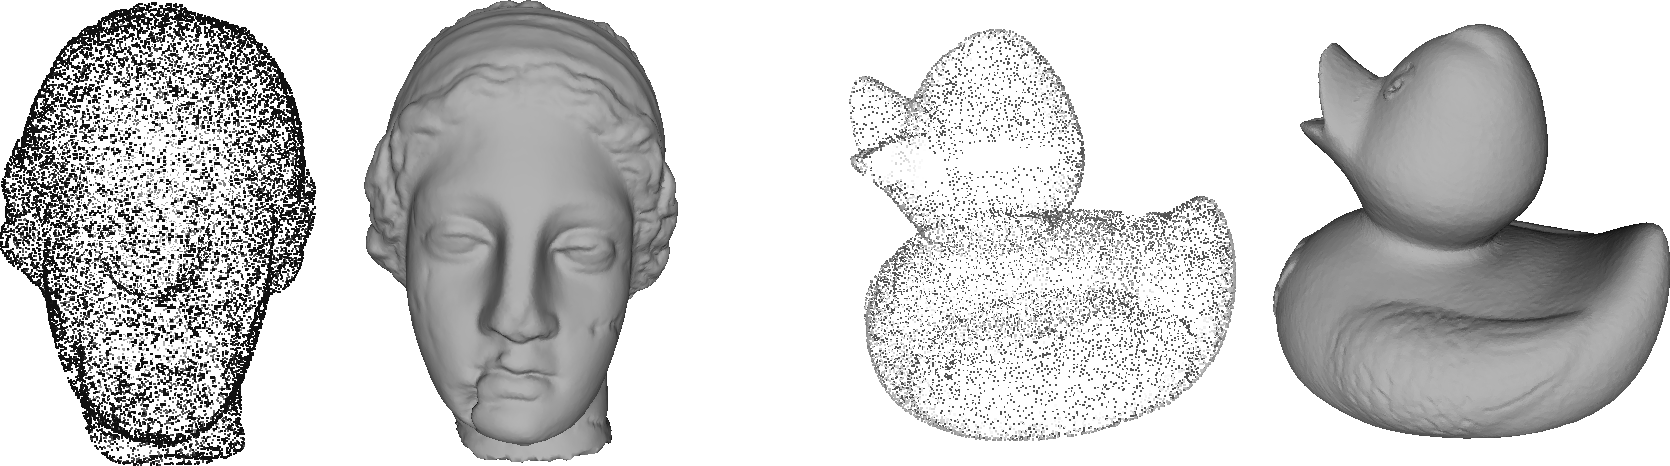
\includegraphics[width=1\linewidth]{images/point_cloud.png}
		\caption{Point Clouds and their reconstructed surfaces. \cite{fig:pc}}
		\label{fig:pointcloud}
	\end{center}
\end{figure}

\subsection{GPU-Voxels Prerequisites}
The GPU-Voxel Algorithm depends on several other Libraries which need to be installed in order to be able to compile GPU-Voxels. The following packages are necessary and must be available:

\setstretch{1.5}
\begin{itemize}
	\item \textbf{nVidia CUDA version 5.5 or higher} \newline CUDA enables many computing cores in a graphics processor to perform general-purpose mathematical calculations, which leads to dramatic speedups in computing performance.
	\item \textbf{Point Cloud Library (PCL)} \newline The Point Cloud Library is an open source library for 2D and 3D image and point cloud processing.
	\item \textbf{OpenNI} \newline OpenNI is an open source software development kit (SDK) used for applications for depth sensors such as Kinect and Asus Xtion.
	\item  \textbf{Boost} \newline Boost is a set of libraries for C++ that provides support for tasks and structures in linear algebra, pseudorandom number generation, multithreading and image processing. It contains over eighty individual libraries which are aimed at a wide range of C++ users.
	\item  \textbf{TinyXML} \newline TinyXML is an XML parser which converts data from an XML format in an in-memory form and creates a way for programs to use that data.
\end{itemize}
\setstretch{1.5}

In order to use the Visualizer further packages are necessary, but in a first installation they are not required and therefore not described in detail.
Installing the necessary packages, has proven difficult because some of them weren't compatible with each other. Sadly, no screenshots of the error message have been taken when occurred and are therefore now not available to be shown in this documentation. This is a finding, which the author now keeps in mind for the documentation of the Bachelor Thesis. 
While installing the nVidia CUDA Toolkit 10.0 the first time. Somehow the graphics driver was damaged, and a simple re-installation of the graphics driver didn't fix it. So, this led to a complete system re-install, with wiping the current Ubuntu partition and starting from Scratch.
In a second attempt all packages could be installed, and the only task left was compiling the GPU-Voxels algorithm. While compiling, cmake had problems finding packages, which was a time consuming but not unsolvable problem. During the step of fixing the package location in the cmake files of the GPU-Voxel Algorithm, several missing packages have been found. Most of them related to Robot operating System (ROS). ROS is an open-source operating System for robotics, which provides common functionality and services used in robotics. While GPU-Voxels state that their algorithm is independent from ROS, but it is supporting it, it was never possible to compile the code without ROS. Some of these packages were found as standalone packages, but couldn't be installed because of unmet dependencies, which lists several other packages and states that they are not going to be installed. This error could be avoided using the packages included in ROS. After installing the ROS Package, the graphics driver was damaged again. This lead again, to a clean start with a fresh Ubuntu installation, because a reinstallation of the graphics driver wouldn't fix the Problem.
In the third attempt the installation order of the packages was changed, and ROS was installed right after CUDA. Afterwards the other necessary packages were installed and compiling the GPU- Voxels Algorithm could start again. As before, some packages were still missing, but could not be installed because of unmet dependencies.
This whole process of trying to run the GPU-Voxels algorithm, was very time consuming and frustrating. A major mistake was, to lose focus on the whole project and how much time had already passed. In this process a lot of time was wasted without getting any results or achieving something. This phase made clear that the planning phase had failed, and the approach to the project was too straight forward directed to the main goal. Together with the missing documentation of the detailed errors and solutions, this Problem had a major influence on not being able to reach the set goals of this preliminary study.

\section{Looking for alternatives}
\label{chap:alternatives}
\setstretch{1.25}

After the struggles with the installation of the packages reached a critical point in terms of time that passed, a decision about the next steps had to be taken. Possible alternatives which allow a progress in this project needed to be found.

As a first step, the task which should be completed by the GPU-Voxel algorithm was divided in different functionalities. Functionality one is, that the workspace needs to be scanned and processed. Functionality two is, that the data from the workspace needs to be compared with the robot model and its trajectories, to predict collisions. Using the data from the collision prediction, a motion planning has to take place in order avoid collisions. To achieve these functionalities the search for packages began by looking into the packages the GPU-Voxel algorithm uses to solve these tasks. A few of them sounded promising, but the search was widened to other standalone libraries for each task to ensure a profound research with the best solution possible. The most promising ones are shortly explained in the following sections.

\subsection{Point Cloud Library \cite{Rusu_ICRA2011_PCL}}
The Point Cloud Library (PCL) supports the Microsoft Kinect cameras as well as the Asus Xtion Pro, which are available for this project. With this library it should be possible to create the necessary point clouds and process them into an octree data structure. The octree data structure was already mentioned in the documentation of the GPU-Voxels algorithm. PCL also provides efficient search routines.

\subsubsection{Octree data structure}

The octree is a tree data structure in which each internal node has exactly eight children. The root node describes a cubic bounding box which encapsulates all points from the point cloud. By
dividing this cube into eight smaller cubes each representing a certain part of the root cube. The node is always the center point of the cube it is representing. Processing a point cloud into an octree data structure already provides a form of voxelizing, the resolution can be chosen by defining how many layers the octree data structure should have.

\begin{figure}[!ht]
	\centering
	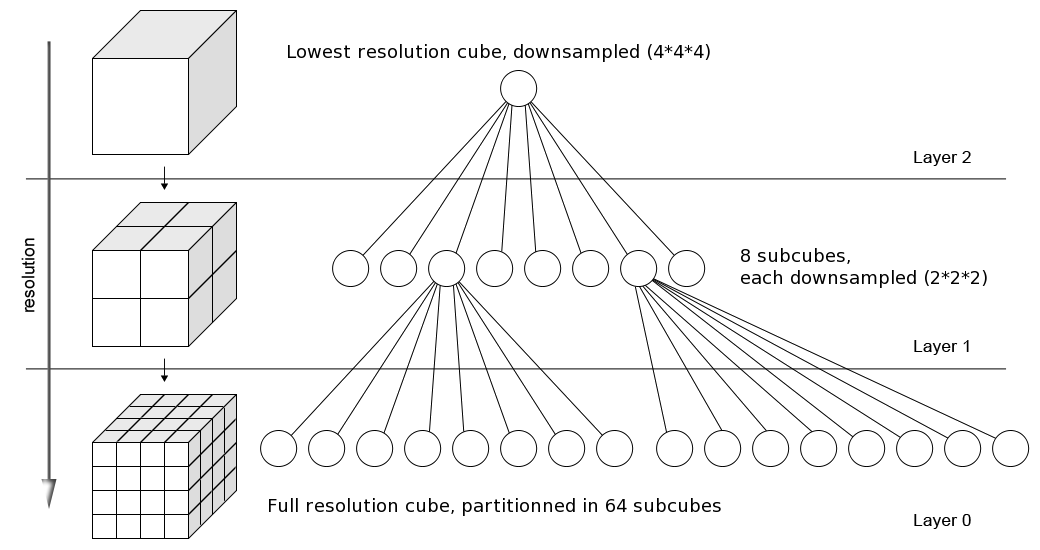
\includegraphics[width=0.6\linewidth]{images/Octree.png}
	\caption{Graphical Illustration of an octree data structure. \cite{fig:octree}}
	\label{fig:octree}
\end{figure}

\subsection{OctoMap \cite{hornung13auro}}
The Octomap library implements a 3D occupancy grid mapping approach, providing data structures and mapping algorithms in C++ suited for robotics. The implementation of the map is based on the previously explained octree data structure, which further allows map-based motion planning to take place.

\subsection{Open Motion Planning Library \cite{sucan2012the-open-motion-planning-library}}
The Open Motion Planning Library (OMPL) consists of many state-of-the-art sampling based motion planning algorithms, but does not contain anything related to collision checking or visualization. So, to use these motion planning algorithms, the collision detection needs to happen before the motion planning and the data needs to be provided accordingly. 

\section{Fanuc Roboguide and TCP/IP Socket messaging}
\label{chap:tcpip}
\setstretch{1.25}
\subsection{Roboguide}
Fanuc has its own simulation software for Fanuc robots called Roboguide. Roboguide provides the user with a complete and realistic simulation of the robot including teach pendant controls of robots. It can also be used to write the Karel programs, which will be later executed from the robot. With Roboguide, every aspect of the robot handling should be able to be simulated, including TCP/IP connections. Simulations are done in workcells, where a robot model can be included and an environment representing the actual robots environment can be created. So as a first step to learn how to use Roboguide, a new workcell was created, which was held very simple only including the robot model. Since it was said that the current physical environment of the robot was going to change in the near future, the work to model the current state was postponed till after the changes has been realized. After including the robot model into the workcell, a simple Karel program was written to move the Robot in a rectangular shape. This code has just been written, to learn some basic Karel functionality and syntax.

\subsection{TCP/IP}

As a first step, the existing work of a former student, Nino Sutter, has been analyzed. The work was provided via a gitlab repository, where access was granted as his work has showed similarities. The code provided should act as an example on how to enable a TCP/IP connection with the robot. The example has a Karel code which connects the robot with a system running a python program. Using the python program, tasks for the robot could be loaded remotely from the memory of the robot. A similar procedure is planned for this thesis. In order to provide the robot with coordinates for his destination point, a C++ program should calculate these and send them to the robot for movement commands. Technically it should be possible to adapt the Karel code from Nino Sutter to achieve the TCP/IP connection for this project on the Fanuc robot.
A first attempt using the example code to simulate a TCP/IP connection within Roboguide has not been successful. The reason for that may be found in missing settings inside the project work cell. But this was not further investigated due to timely limits of the preliminary study and the problems which occurred during GPU-Voxel algorithm setup.
Alternatively, the AHB has currently socket messaging, which is working on the robot for another project. This method of communication has not yet been reviewed, since the information came up in week 11 which is too close to the end of the preliminary studies due date. During the Bachelor Thesis this will be further analyzed to make sure to use the communication method that fits best \cite{motion}.



\chapter{Planning of the Bachelor Thesis}
\label{chap:planning}
\setstretch{1.25}

To have small and achievable goals to work on during the Bachelor Thesis, the project is divided in several milestones. In this chapter these milestones are listed and explained in detail on what is the goal, what are the methods used to achieve it, how is it tested and how to proof that they worked. The milestones will start from a few that are necessary to have the bare minimum done and will go up until the optimal solution. After the milestones were described, predictions are made on how far the project will be solved under different circumstances (e.g. worst-case scenario, no problems etc.).

\section{Milestone 1: Running programming environment}
\label{chap:mile1}
\subsubsection{Description}
Until this point of time, the work for this project was completely done on private systems of the student. As mentioned in chapter 4 a laptop was provided by the AHB. Since it is a school laptop, a Windows system is installed. In order to not uninstall the Windows off the Laptop, an external SSD was provided which should be configured to act as a bootable Ubuntu 18.04 Bionic Beaver System. Therefore, the system will start again from a clean installation and all needed libraries will be installed on to this system.
\subsubsection{Goal}
The Goal is straightforward to have a running programming environment which has all needed libraries and programs installed.
\subsubsection{Methods used to achieve the goal}
Following installation instructions of different libraries which are offered by the providers of the needed libraries.
\subsubsection{Testing}
Ubuntu is bootable from multiple Devices.
The boot will be tested on at least two different devices. 
\subsubsection{Validation and proof}
The device allows a flawless boot of the Ubuntu into the desired home screen without changing the predefined setups.
Proof is a written statement of the user / author.

\section{Milestone 2: Robot communication}
\label{chap:mile2}
\subsubsection{Description}
Without the communication with the robot, the task of the project can't be achieved. Therefore it is very important to set up a stable connection and communication from the system to the robot in order to provide each side of the system with the necessary data.
\subsubsection{Goal}
Flawless communication between collision avoidance system and robot.
\subsubsection{Methods used to achieve the goal}
Review the example provided over git and the socket messaging method already in use at AHB. Work with the Fanuc manual in order to set up the communication.
\subsubsection{Testing}
In order to test the communication, a simple C++ program should be able to feed the robot Cartesian or joint coordinates to move to. The robot shall move accordingly.
\subsubsection{Validation and proof}
The C++ as well as the Karel code shall be pushed to git in a separate folder, to provide a simple example for future communication tasks.
A video shall be provided as proof for the functioning communication. The video shall show the execution of the C++ code and the robot's movements. The video and the source code will be committed in a single commit in order to have a  clear identification.

\section{Milestone 3: Scanning of the workspace}
\label{chap:mile3}
\subsubsection{Description}
The cameras shall be implemented into the system and a point cloud of the Workspace shall be created. The data shall be processed into a two-dimensional occupancy grid for a first simple motion planner.
\subsubsection{Goal}
Visualizing the workspace in form of a point cloud and an occupancy grid.
\subsubsection{Methods used to achieve the goal}
Using the Point Cloud Library, the cameras shall be implemented. Since the PCL supports either Microsoft Kinect or Asus Xtion Pro, both cameras may be used, the one with the better resulsts shall be used for the rest of the project.
\subsubsection{Testing}
In order to test the task, the workspace shall be changed by placing different objects on various points inside the workspace.
Point clouds and occupancy grids will be reviewed manually and checked for their accuracy.
\subsubsection{Validation and proof}
The successful test will be proceeded and documented with both kinds of cameras.
The resulting grids are analyzed manually and a ranking for completeness and accuracy will be done.
Proof shall be provided over screenshots and written comments of the observation and usability of the author.

\section{Milestone 4: Simple 2D Motion Planning, End-Effector only}
\label{chap:mile4}
\subsubsection{Description}
In a first collision avoidance step, the robot shall move around objects in a static two dimensional environment. This means during robot movements the workspace shall not change. A simple algorithm for path planning is the PRM algorithm, which should be available over the Open Motion Planning Library. PRM is already known since it was used during the robotics 2 course. In this course an implementation was realized over Matlab.
\subsubsection{Goal}
Move from start position to given goal position without any collision.
\subsubsection{Methods used to achieve the goal}
The point clouds gathered from the cameras using PCL, shall be processed into an 2D occupancy grid using OctoMap. The probabilistic road map planner (PRM) uses occupancy grids and places nodes inside the map on randomly chosen free cells. The nearest nodes to the starting and goal location are searched. Then a path along the nodes is calculated and thus provides a path from start to goal position. The PRM planner can be used from the OMPL library.
This step plans the motions only for the end-effector, which means the robot arm needs to remain elevated over the obstacles in order to remain collision free. Therefor movements can only be made in the XY-plane in Cartesian space.
\subsubsection{Testing}
By changing the workspace with different objects on various places, the map generation and the path planning shall be tested. The starting position shall be read from the Karel code as the current robot position, the goal position shall be provided over the C++ Code as an user input.
\subsubsection{Validation and proof}
Three successful test runs with different objects in different positions and variable start and end points shall be proceeded.
A video of the robot's movement around the object shall be made for every run to proof that the path planning works in different test set-ups.

\section{Milestone 5: Simple 3D Motion Planning, End-Effector only}
\label{chap:mile5}
\subsubsection{Description}
As a second collision avoidance step, the robot shall move around in a static three dimensional environment. The objects inside the workspace shall remain static during robot movements. For the motion planning, again the PRM algorithm shall be used, but this time in a 3D space.
\subsubsection{Goal}
Move from start position to given goal position without any collision in the three dimensional space.
\subsubsection{Methods used to achieve the goal}
The point clouds gathered from the cameras using PCL, shall be processed into an 3D occupancy grid using OctoMap. Using the PRM planner from OMPL a path from start to goal shall be calculated and afterwards moved along with the robot.
This step plans the motions only for the end-effector, which means the robot arm needs to remain elevated over the obstacles in order to remain collision free. Therefor movements can only be made in the Cartesian space.
\subsubsection{Testing}
By changing the workspace with different objects on various places, the map generation and the path planning shall be tested. The starting position shall be read from the Karel code as the current robot position, the goal position shall be provided over the C++ Code as an user input.
\subsubsection{Validation and proof}
Three successful test runs with different objects in different positions and variable start and end points shall be proceeded.
A video of the robot's movement around the object shall be made for every run to proof that the path planning works in different test set-ups.

\section{Milestone 6: Collision detection for whole robot model}
\label{chap:mile6}
\subsubsection{Description}
The next step to improve the collision avoidance system shall provide a collision detection not only for the end-effector but for the whole robot model. This shall be achieved by creating a occupancy grid for the robot model and its trajectories. By comparing the two different grids (workspace and robot) collisions shall be predicted and avoided.
\subsubsection{Goal}
Find or create a motion planner who is able to calculate a path based on swept volumes. 
Move from start position to given goal position without any collision, movements can be done in joint space or Cartesian space.
\subsubsection{Methods used to achieve the goal}
A 3D model of the robot provides the base for the robot occupancy grid. Using the joint speeds, a prediction of the joint positions can be calculated and swept volumes can be created inside the occupancy grid. Both occupancy grids shall be compared by simply checking if a cell is occupied in both grids. The cells which are occupied in both grids show a collision that needs to be avoided.
To have a proper motion planning algorithm based on these data, further literature review is necessary.

\subsubsection{Testing}
The workspace shall be changed for different motions by placing various objects in different positions. In order to test the collision detection for the robot arm, objects shall be placed in front of the arm to force a movement to avoid the collision not only of the end-effector.

\subsubsection{Validation and proof}
Three successful test runs with different objects in different positions and variable start and end points shall be proceeded.
A video of the robot's movement around the object shall be made for every run to proof that the path planning works in different test set-ups.

\section{Milestone 7: Collision detection in a dynamic workspace}
\label{chap:mile7}
\subsubsection{Description}
The previously used motion planner shall be adapted to work in a dynamic workspace (e.g. moving objects, humans). The movements of the robot shall be adapted in real time to avoid collisions. The results of the collision avoidance system shall be visualized in a GUI. 


\subsubsection{Goal}
Robot moves from start to goal location in a dynamic workspace, without any collisions.
Implement a GUI to show the results of the collision avoidance system.

\subsubsection{Methods used to achieve the goal}
The workspace shall be monitored in real-time, updating occupancy grids on the fly. The motion planner should work with the permanently updating occupancy grids in order to react to dynamic obstacles.
Further literature review is necessary to achieve this goal.

\subsubsection{Testing}
In a first phase, object shall be moved inside the workspace, using objects which can be moved from outside of the workspace to reduce risks for humans.
In a second phase, when the system has a high level of success an values can be considered as trustworthy, humans shall enter and leave the workspace in order to simulate a walk by.

\subsubsection{Validation and proof}
Six successful test runs with different objects in various positions and variable start and end points shall be proceeded by using objects which are moved from outside of the workspace.
A video of the robot's movement around the object shall be made for every run to proof that the path planning works in different test set-ups. 
After the successful first testing phase another three test runs with humans shall be proceeded and recorded on video. 

\section{Prediction}

Milestones one to four are defined as bare minimum, as these are the necessary milestones to have a first path planning based on the sensor data, which implements a first step of the collision avoidance system. Based on the actual knowledge it should be possible to reach Milestone six within the given eight weeks of the Bachelor Thesis. If progress during the work is exceptionally good, even milestone seven can be reached.

To prevent the lost of track, an escalation to the experts is needed, whenever the forseen timeline of the worst case is not fulfilled. This would mean, that the minimal goal is threatened and a solution to this upcoming problem need to be found. In addition it helps the author to prevent losing focus as it happened in the preliminary study.

\begin{figure}[h]
	\begin{center}
		\centering
		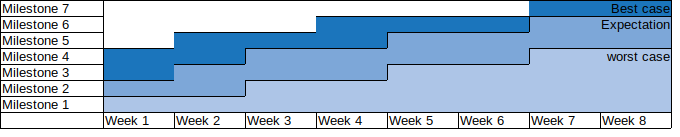
\includegraphics[width=1.0\linewidth]{images/Milestones.png}
		\caption{Milestones in Timeline}
		\label{fig:milestones}
	\end{center}
\end{figure}
\chapter{Conclusion / Results}
\label{chap:conclusions}
Overall the process of the preliminary study did not work out as expected. On one hand the technical requirements for the programming environment caused way more problems than expected and on the other hand, the time planning and focus of the author did get out of hand. The combination of these two issues caused major time and motivation problems. Therefore the result of the preliminary study is not satisfying for the author in accordance to the initial expectation.
Nevertheless, working on this project is very interesting and challenging, which means that the will to continue this project is unbroken.

Content wise there should have been a bigger accomplishment according the time given and the massive amount of time invested. After many hours of literature review, a sobering low amount of portable possibilities has been found. This leads to the conclusion that the way of research has to be adapted in order to find suitable solution for the existing issues.
Due to the adaption of the initial plan and the exchange with the experts, a realistic approach has been defined. Under consideration of all these factors, the best possible result is now provided.

The most important learning for the work on the milestones is to keep an strong focus on the actual tasks combined with a good and mindful time management. Also the exchange with other students and the experts shall be kept alive to benefit of the given knowledge. Help shall be searched at a earlier point of time, which does not mean, not to try to fix problems by the authors own possibilities and serious tries.

The definition of the milestones provides a promising planning of the Bachelor Thesis and seems to allow a good result for the main goal of the project. Needed Hardware and Software is mostly identified and methods to fulfill the requirements are described. 

An intense research of the topic and possible alternatives for occurred problems has been executed and leads to a knowledge which can be used and extended during the Bachelor Thesis.  

For the start of the Bachelor Thesis, only the learning will be taken into account and the disappointment is left behind. With great motivation and a strong will to perform well, the author is now looking forward to the realization of the milestones of the Bachelor Thesis. 
%---------------------------------------------------------------------------

% Selbst�ndigkeitserkl�rung
%---------------------------------------------------------------------------
%\cleardoublepage
%\phantomsection 
\addcontentsline{toc}{chapter}{Declaration of authorship}
\chapter*{Declaration of primary authorship}
\label{chap:declaration_authorship}

\vspace*{10mm} 

I hereby confirm that I have written this thesis independently and without using other sources and resources than those specified in the bibliography. All text passages which were not written by me are marked as quotations and provided with the exact indication of its origin. 

\vspace{15mm}

\begin{tabbing}
xxxxxxxxxxxxxxxxxxxxxxxxxxxxxx\=xxxxxxxxxxxxxxxxxxxxxxxxxxxxxx\=xxxxxxxxxxxxxxxxxxxxxxxxxxxxxx\kill
Place, Date:		\> Biel, \versiondate \\ \\ 
Last Name, First Name:	\> Aeschlimann, Dario 	\>  \\ \\ \\ \\ 
Signature:	\> ......................................\> ...................................... \\
\end{tabbing}

%---------------------------------------------------------------------------

% Glossary
%---------------------------------------------------------------------------
%\cleardoublepage
%\phantomsection 
%\addcontentsline{toc}{chapter}{Glossary}
%\renewcommand{\glossaryname}{Glossay}
%\printglossary
%---------------------------------------------------------------------------

% Bibliography
%---------------------------------------------------------------------------
%\cleardoublepage
%\phantomsection 
\addcontentsline{toc}{chapter}{Bibliography}
\bibliographystyle{IEEEtranS}
\bibliography{database/bibliography}{}
%---------------------------------------------------------------------------

% Listings
%---------------------------------------------------------------------------
%\cleardoublepage
%\phantomsection 
\addcontentsline{toc}{chapter}{List of figures}
\listoffigures
%\cleardoublepage
%\phantomsection 
%\addcontentsline{toc}{chapter}{List fo tables}
%\listoftables
%---------------------------------------------------------------------------

% Index
%---------------------------------------------------------------------------
%\cleardoublepage
%\phantomsection 
\addcontentsline{toc}{chapter}{Index}
\printindex
%---------------------------------------------------------------------------

% Attachment:
%---------------------------------------------------------------------------
%\appendix
%\settocdepth{section}
%\chapter*{APPENDICES}
\addcontentsline{toc}{chapter}{APPENDICES}

\begingroup\let\clearpage\relax
\chapter{Arbitrary Appendix}
\label{chap:appendix_arb}
\endgroup

The European languages are members of the same family. Their separate existence is a myth. For science, music, sport, etc, Europe uses the same vocabulary. The languages only differ in their grammar, their pronunciation and their most common words. Everyone realizes why a new common language would be desirable: one could refuse to pay expensive translators. To achieve this, it would be necessary to have uniform grammar, pronunciation and more common words. If several languages coalesce, the grammar of the resulting language is more simple and regular than that of the individual languages. The new common language will be more simple and regular than the existing European languages. It will be as simple as Occidental; in fact, it will be Occidental. 
%\chapter{Additional Appendix}
\label{chap:appendix_B}

\section{Test 1}
To an English person, it will seem like simplified English, as a skeptical Cambridge friend of mine told me what Occidental is. The European languages are members of the same family. Their separate existence is a myth. For science, music, sport, etc, Europe uses the same vocabulary. The languages only differ in their grammar, their pronunciation and their most common words. Everyone realizes why a new common language would be desirable: one could refuse to pay expensive translators. To achieve this, it would be necessary to have uniform grammar, pronunciation and more common words. If several languages coalesce, the grammar of the resulting language is more simple and regular than that of the individual languages. The new common language will be more simple and regular than the existing European languages. 

\subsection{Environment}
It will be as simple as Occidental; in fact, it will be Occidental. To an English person, it will seem like simplified English, as a skeptical Cambridge friend of mine told me what Occidental is. The European languages are members of the same family. Their separate existence is a myth. For science, music, sport, etc, Europe uses the same vocabulary. The languages only differ in their grammar, their pronunciation and their most common words. Everyone realizes why a new common language would be desirable: one could refuse to pay expensive translators. To achieve this, it would be necessary to have uniform grammar, pronunciation and more common words.
%---------------------------------------------------------------------------

%---------------------------------------------------------------------------
\end{document}

